\documentclass[11pt, a4paper, oneside]{book}

% URLs and hyperlinks ---------------------------------------
\usepackage{hyperref}
\hypersetup{
	colorlinks=true,
	linkcolor=blue,
	filecolor=magenta,      
	urlcolor=blue,
}
\usepackage[inline]{enumitem}
\usepackage{xurl}
%---------------------------------------------------


% code snippet -------------------------------------------------------
\usepackage{minted}
% ---------------------------------------------------------------------

% page headers -------------------------------------------------
\usepackage{fancyhdr}
\fancypagestyle{plain}{\fancyhf{}\renewcommand{\headrulewidth}{0pt}}
\pagestyle{fancy}
\fancyhf{}% Clear header/footer
\fancyhead[L]{\nouppercase\leftmark}
\fancyhead[R]{\thepage}
%---------------------------------------------------------------

% adjust a verrrrry big table -------------------------------
\usepackage{adjustbox}
% -----------------------------------------------------------

% titlepage -------------------------------------------------
\usepackage{pdfpages}
%------------------------------------------------------------
% titlepage -------------------------------------------------
\usepackage{svg}
%------------------------------------------------------------
% sudo apt inkscape
% command: pdflatex --shell-escape


% titlepage -------------------------------------------------
\usepackage[font=small,labelfont=bf]{caption}
%------------------------------------------------------------


% Rn custom item in enumeration -----------------------------
\newcounter{itemadded}
\setcounter{itemadded}{0}


\newcommand{\addeditem}{%
	\addtocounter{enumi}{-1}%
	\stepcounter{itemadded}
	\let\LaTeXStandardLabelEnumi\labelenumi%
	\addtocounter{enumi}{1}
	\renewcommand{\labelenumi}{\arabic{enumi}\lr{R}.}%
	\item 
	% Switch back to old labelling 
	\let\labelenumi\LaTeXStandardLabelEnumi%
}%


\let\LaTeXStandardEnumerateBegin\enumerate
\let\LaTeXStandardEnumerateEnd\endenumerate

\renewenvironment{enumerate}{%
	\LaTeXStandardEnumerateBegin%
	\setcounter{itemadded}{0}
}{%
	\LaTeXStandardEnumerateEnd%
}%
% -----------------------------------------------------------

% tables -------------------------------------------------------
\usepackage{float}
\usepackage{multirow}
\renewcommand{\arraystretch}{1.23}
% ---------------------------------------------------------------------

\usepackage{xepersian}
\settextfont{Yas}
\setdigitfont{Yas}
\setlatintextfont{Yas}

\usepackage{minted}

\begin{document}
	\frontmatter
	
	\begin{titlepage}
		\centering
		\includesvg[width=4cm]{./layout/besm}\par
	
		\vspace{1cm}
    \includesvg[width=3.2cm]{./layout/logo}\par % Do not include the .svg extension
		
		\vspace{5mm}
		{\LARGE دانشگاه اصفهان}\par
		\vspace{5mm}
		{\Large دانشکده مهندسی کامپیوتر}\par
		
		\vspace{2cm}
		
		{\Large فاز اول پروژه در مبانی هوش و کاربردها}\par
		\vspace{1cm}
		{\Huge پک‌من و رگرسیون خطی}\par
		
		
		\vspace{2cm}
		{\Large استاد درس: دکتر حسین کارشناس}\par
		\vspace{0.5cm}
		{\Large دستیار استاد: پوریا صامتی}
		
		\vspace{1.2cm}
		{\Large دانیال شفیعی}\par
		{\Large مهدی مهدیه}\par
		{\Large سید امیررضا نجفی}\par
		
		\vspace{2cm}
		
		% Bottom of the page
		{\large آبان ۱۴۰۳\par}
	\end{titlepage}
	\tableofcontents
	\newpage
	\mainmatter
	
	\chapter{Pacman}
	هدف از پیاده‌سازی این بخش از پروژه این است که با جستجو مسیری بهینه (از لحاظ فاصله طی شده و همچنین تعداد گره‌های جستجو شده) پیدا کنیم که در آن پک‌من بتواند همه‌ی غذاها را بخورد.
	\section{توابع جستجوی مسیر}
	همانطور که در پروژه گفته شد ما از چهار آلگوریتم  عمق اول و عرض اول، هزینه‌یابی یکنواخت و  
	\lr{$A^{\star}$}
	 استفاده کردیم.
	 
	 \subsection{تابع عمق اول}
	 در این تابع هدف پیدا کردن مسیر خوردن اهداف به نحوی است که کمترین گره را جستجو کنیم. در این تابع الزاما مسیر پیدا شده بهترین مسیر نیست و مشاهده می‌شود پک‌من از بیراهه می‌رود. کد پیاده‌سازی این تابع:
	 \begin{LTR}
\begin{minted}[frame=lines, fontsize=\small, tabsize=4, texcomments=false]{python}
q = util.Stack()
empty_action_list = []
visited = set()
q.push((problem.getStartState(), empty_action_list))
visited.add(problem.getStartState())
while not q.isEmpty():
    current_node, list_of_actions = q.pop()
    if problem.isGoalState(current_node):
        return list_of_actions
    for info in problem.getSuccessors(current_node):
        successor, action, step_cost = info
        if successor not in visited:
            new_list = list_of_actions + [action]
            q.push((successor, new_list))
            visited.add(successor)
\end{minted}
	 \end{LTR}
	
		 \subsection{تابع عرض اول}
	در این تابع هدف پیدا کردن مسیر خوردن اهداف به نحوی است که بهترین مسیر را جستجو کنیم. در این تابع الزاما تعداد گره‌های جستجو شده بهینه‌ترین حالت نیست. اما بعد از اینکه کد آن اجرا شد پک‌من از کوتاه‌ترین مسیر به مقصد می‌رسد. کد پیاده‌سازی این تابع:
	\begin{LTR}
		\begin{minted}[frame=lines, fontsize=\small, tabsize=4, texcomments=false]{python}
q = util.Queue()
empty_action_list = []
visited = set()
q.push((problem.getStartState(), empty_action_list))
visited.add(problem.getStartState())
while not q.isEmpty():
    current_node, list_of_actions = q.pop()
    if problem.isGoalState(current_node):
        return list_of_actions
    for info in problem.getSuccessors(current_node):
        successor, action, step_cost = info
        if successor not in visited:
            new_list = list_of_actions + [action]
            q.push((successor, new_list))
            visited.add(successor)
		\end{minted}
	\end{LTR}
	
	
	\subsection{تابع هزینه‌یابی یکنواخت}
	در این تابع هدف پیدا کردن مسیر خوردن اهداف به نحوی است که بهترین مسیر را جستجو کنیم به نحوی که در آن ممکن است طی کردن هر مسیر هزینه‌ی مشخصی داشته باشد. تفاوت این تابع با تابع جستجوی عرض اول در همین دخیل کردن هزینه‌هاست. کد پیاده‌سازی این تابع:
\begin{LTR}
\begin{minted}[frame=lines, fontsize=\small, tabsize=4, texcomments=false, breaklines=true, breakanywhere=true]{python}
priority_queue = util.PriorityQueue()
start_state = problem.getStartState()
priority_queue.push((start_state, []), 0)
visited = set()

while not priority_queue.isEmpty():
    state, actions = priority_queue.pop()

    if problem.isGoalState(state):
        return actions

    if state not in visited:
        visited.add(state)

        successors = problem.getSuccessors(state)
        for successor, action, cost in successors:
            if successor not in visited:
                new_cost = problem.getCostOfActions(actions + [action])
                priority_queue.push((successor, actions + [action]), new_cost)
\end{minted}
\end{LTR}
	
	
	
	\subsection{تابع \lr{$A^{\star}$}}
	در این تابع هدف پیدا کردن مسیر خوردن اهداف به نحوی است که هم بهترین مسیر را جستجو کنیم و هم تعداد گره‌های جستجو شده را کاهش دهیم. به این منظور ما هر بار یک تخمین . تفاوت این تابع با تابع جستجوی عرض اول در همین دخیل کردن هزینه‌هاست. کد پیاده‌سازی این تابع:
\begin{LTR}
	\begin{minted}[frame=lines, fontsize=\small, tabsize=4, texcomments=false,
		breaklines=true, breakanywhere=true]{python}
heuristic = cornersHeuristic
priority_queue = util.PriorityQueue()
start_state = problem.getStartState()
priority_queue.push((start_state, []), 0)
visited = set()

while not priority_queue.isEmpty():
    state, actions = priority_queue.pop()

    if problem.isGoalState(state):
        return actions

    if state not in visited:
        visited.add(state)

        successors = problem.getSuccessors(state)
        for successor, action, cost in successors:
            if successor not in visited:
                new_cost = problem.getCostOfActions(actions + [action])
                priority_queue.push((successor, actions + [action]), new_cost + heuristic(successor, problem))

	\end{minted}
\end{LTR}
 که در آن تابع cornerHeuristic را بدین نحو پیاده‌سازی کرده‌ایم:
 \begin{LTR}
 	\begin{minted}[frame=lines, fontsize=\small, tabsize=4, texcomments=false,
 		breaklines=true, breakanywhere=true]{python}
 position, corner = state
 corners = problem.corners
 unseens = [corner1 for i, corner1 in enumerate(corners) if not corner[i]]
 
 if len(unseens) == 0:
     return 0
 sum1 = 0
 for current_corner in unseens:
     sum1 = sum1 + util.manhattanDistance(position, current_corner)
 return sum1 * len(unseens) * 2
 	\end{minted}
 \end{LTR}
	باید دقت نمود این تابع یک اکتشاف غیر قابل قبول 
	\footnote{Non-Adimissible} 
	است. البته این به خودی خود ایرادی ایجاد نمی‌کند. علت اینکه تابع ما غیر قابل قبول است این است که ضرب تعداد غذاها در مجموع فاصله‌ی منهتنی می‌تواند بیشتر از فاصله‌ی واقعی باشد. 
	
	
	علت اینکه  sum را ضربدر تعداد غذاعا کردیم  این بود که هر بار هنگامی که یکی از اهداف را می‌خورد، تخمین مقدار قابل توجهی کاهش می‌یافت و به نوعی به الگوریتم می‌فهماند که خوب عمل کرده است. مثلا در حالتی که پک‌من در وسط صفحه قرار داشته باشد و دو غذا در بالا چپ و پایین راست، با شرایطی که هر دو فاصله مساوی از پک‌من داشته باشند و پک‌من یکی از آنها را بخورد، تابع اکتشاف هنوز همان مقدار قبلی را برمی‌گرداند زیرا جمع فاصله‌ی منهتنی از غذاها تغییری نکرده است. اما در شرایطی که تعداد را دخیل کنیم باعث می‌شود  مقدار تابع اکتشاف پس از خوردن یک هدف کاهش پیدا کند.
	
	
	
	
	
	
	
	
	
\section{خروجی توابع}
در این بخش خروجی هر تابع را در محیط‌های مختلف گزارش می‌کنیم.
	\begin{center}
	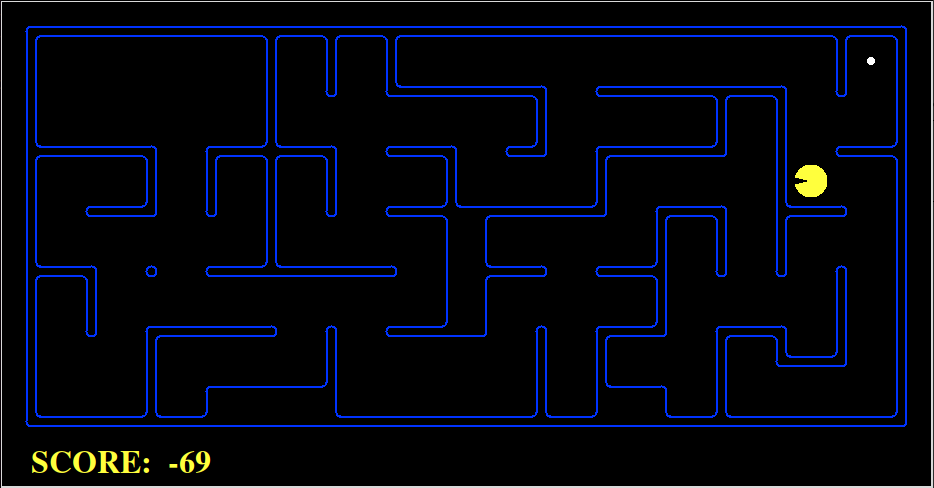
\includegraphics[width=10cm]{./images/pacman.png}
	\captionof{figure}{محیط گرافیکی بازی پک‌من}
\end{center}
	 \subsection{محیط ساده}
\begin{LTR}
	\begin{minted}[frame=lines, fontsize=\small, tabsize=4, texcomments=false]{text}
#DFS
[SearchAgent] using function dfs
[SearchAgent] using problem type CornersProblem
Path found with total cost of 32 in 0.0 seconds
Search nodes expanded: 185
Pacman emerges victorious! Score: 478
Average Score: 478.0
Scores:        478.0
Win Rate:      1/1 (1.00)
Record:        Win

#BFS
[SearchAgent] using function bfs
[SearchAgent] using problem type CornersProblem
Path found with total cost of 20 in 0.0 seconds
Search nodes expanded: 225
Pacman emerges victorious! Score: 490
Average Score: 490.0
Scores:        490.0
Win Rate:      1/1 (1.00)
Record:        Win

#UCS
[SearchAgent] using function ucs
[SearchAgent] using problem type CornersProblem
Path found with total cost of 20 in 0.0 seconds
Search nodes expanded: 225
Pacman emerges victorious! Score: 490
Average Score: 490.0
Scores:        490.0
Win Rate:      1/1 (1.00)
Record:        Win

#ASTAR
[SearchAgent] using function astar and heuristic nullHeuristic
[SearchAgent] using problem type CornersProblem
Path found with total cost of 20 in 0.0 seconds
Search nodes expanded: 23
Pacman emerges victorious! Score: 490
Average Score: 490.0
Scores:        490.0
Win Rate:      1/1 (1.00)
Record:        Win
	\end{minted}
\end{LTR}

\subsection{محیط سخت}
\begin{LTR}
	\begin{minted}[frame=lines, fontsize=\small, tabsize=4, texcomments=false]{text}
#DFS
Corner -p SearchAgent  -a fn=dfs,prob=CornersProblem
[SearchAgent] using function dfs
[SearchAgent] using problem type CornersProblem
Path found with total cost of 201 in 0.0 seconds
Search nodes expanded: 340
Pacman emerges victorious! Score: 339
Average Score: 339.0
Scores:        339.0
Win Rate:      1/1 (1.00)
Record:        Win

#BFS
[SearchAgent] using function bfs
[SearchAgent] using problem type CornersProblem
Path found with total cost of 106 in 0.0 seconds
Search nodes expanded: 1966
Pacman emerges victorious! Score: 434
Average Score: 434.0
Scores:        434.0
Win Rate:      1/1 (1.00)
Record:        Win

#UCS
[SearchAgent] using function ucs
[SearchAgent] using problem type CornersProblem
Path found with total cost of 106 in 0.2 seconds
Search nodes expanded: 1966
Pacman emerges victorious! Score: 434
Average Score: 434.0
Scores:        434.0
Win Rate:      1/1 (1.00)
Record:        Win

#ASTAR
[SearchAgent] using function astar and heuristic nullHeuristic
[SearchAgent] using problem type CornersProblem
Path found with total cost of 106 in 0.0 seconds
Search nodes expanded: 187
Pacman emerges victorious! Score: 434
Average Score: 434.0
Scores:        434.0
Win Rate:      1/1 (1.00)
Record:        Win

	\end{minted}
\end{LTR}


\subsection{محیط بزرگ}

\begin{LTR}
	\begin{minted}[frame=lines, fontsize=\small, tabsize=4, texcomments=false, breaklines=true, breakanywhere=true]{text}
#DFS
[SearchAgent] using function dfs
[SearchAgent] using problem type CornersProblem
Path found with total cost of 280 in 0.0 seconds
Search nodes expanded: 900
Pacman emerges victorious! Score: 270
Average Score: 270.0
Scores:        270.0
Win Rate:      1/1 (1.00)
Record:        Win

#BFS
[SearchAgent] using function bfs
[SearchAgent] using problem type CornersProblem
Path found with total cost of 210 in 0.1 seconds
Search nodes expanded: 11392
Pacman emerges victorious! Score: 340
Average Score: 340.0
Scores:        340.0
Win Rate:      1/1 (1.00)
Record:        Win

#UCS
[SearchAgent] using function ucs
[SearchAgent] using problem type CornersProblem
Path found with total cost of 210 in 1.7 seconds
Search nodes expanded: 11392
Pacman emerges victorious! Score: 340
Average Score: 340.0
Scores:        340.0
Win Rate:      1/1 (1.00)
Record:        Win

#ASTAR
[SearchAgent] using function astar and heuristic nullHeuristic
[SearchAgent] using problem type CornersProblem
Path found with total cost of 286 in 0.1 seconds
Search nodes expanded: 969
Pacman emerges victorious! Score: 264
Average Score: 264.0
Scores:        264.0
Win Rate:      1/1 (1.00)
Record:        Win
	\end{minted}
\end{LTR}

\textbf{توضیح:}
 نتیجه امتیاز و تعداد گره‌های جستجو شده  تابع هزینه‌یابی یکنواخت با تابع جستجوی عرض اول یکی است! فقط هزینه‌یابی در زمان جستجو بیشتر است. علت آن این است که هزینه‌ی حرکت به خانه ۱ واحد درنظر گرفته شده و چون تابع هزینه‌یابی یکنواخت روی هزینه‌ها متمرکز است از قضا زمان بسیار بیشتری هم طول کشیده! واضح است که ممکن است در شرایطی که هزینه‌ی رفتن به هر خانه برابر نباشد نتایج متفاوت شوند.

	
	
	
	
	
	
	
	
	
	
	
	\chapter{رگرسیون خطی}
	در این بخش از پروژه ما قصد داشتیم با داده‌های آموز مدلی را بسازیم که با آن داده‌های جدید را پیش‌بینی کنیم. 
	\section{اکتشاف درون داده‌ها}
	با توجه به اینکه همه‌ی ستون‌های ما به جز id متغیرهای پیوسته بودند، ما می‌توانستیم به خوبی خود احتمال را که یک چیز پیوسته است پیش‌بینی کنیم.
	صرفا یک شک درمورد این وجود داشت که idها در میان سطرهای یکی باشند. برای همین این را بررسی کردیم و چنین نبود. بنابرین متغیر id را که یک متغیر categorical بود حذف کردیم. 
	\subsection{پر کردن مقادیر خالی}
	داده‌ها هیچ مقادیر خالی نداشتند اما ما یک تابع
	\lr{knn imputer}
	  نوشتیم که به‌جای میانگین گرفتن از کل داده‌ها از k همسایه‌ نزدیک (با توجه به بقیه‌ی ویژگی‌ها) میانگین می‌گیرد و مقادیر را پر می‌کند. فاصله در این تابع به صورت فاصله‌ی اقلیدسی تعریف شده است.
	در نهایت اما به علت پیچیدگی ما از یک تابع میانگین ساده روی کل مقادیر برای پر کردن داده‌ها استفاده کردیم.
	\subsection{رسم نقشه گرمایی همبستگی}

	\begin{center}
		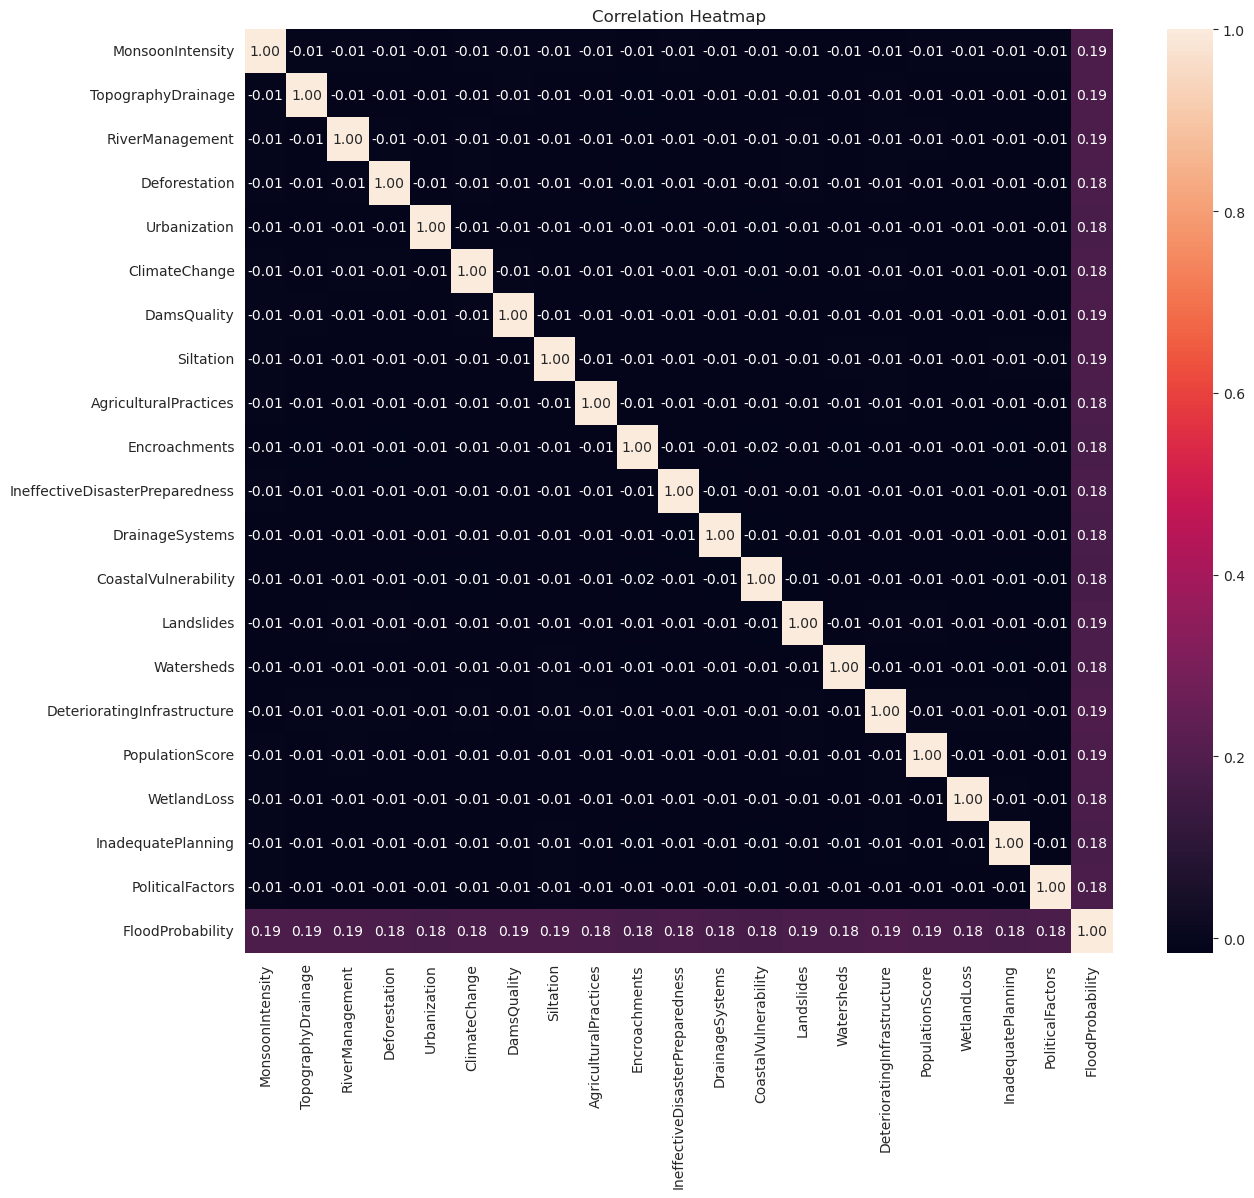
\includegraphics[width=7cm]{./images/heatmap.png}
		\captionof{figure}{نقشه گرمایی همبستگی متغیرها}
\end{center}

	تقریبا هیچ همبستگی بین داده‌ها وجود ندارد تا آن را حذف کنیم. 
	به عنوان یک پیشنهاد ما تست کردیم که اگر دو ستون را در هم ضرب کنیم چه اتفاقی برای همبستگی و همچنین میانگین مربع خطا می‌افتد برای همین در نوتبوک feature.ipynb این قضیه را تست کردیم. این کار را برای همه‌ی ستون‌ها تکرار کردیم و نتیجه همبستگی مقداری بهتر شد. بنابرین ما یک تابع جدید با ضرب بالاترین میانگین همبستگی ایجاد کردیم که البته در ادامه از این کار پشیمان شدیم! (چون در همه‌ی شرایط بدتر عمل می‌کرد)

	\begin{center}
	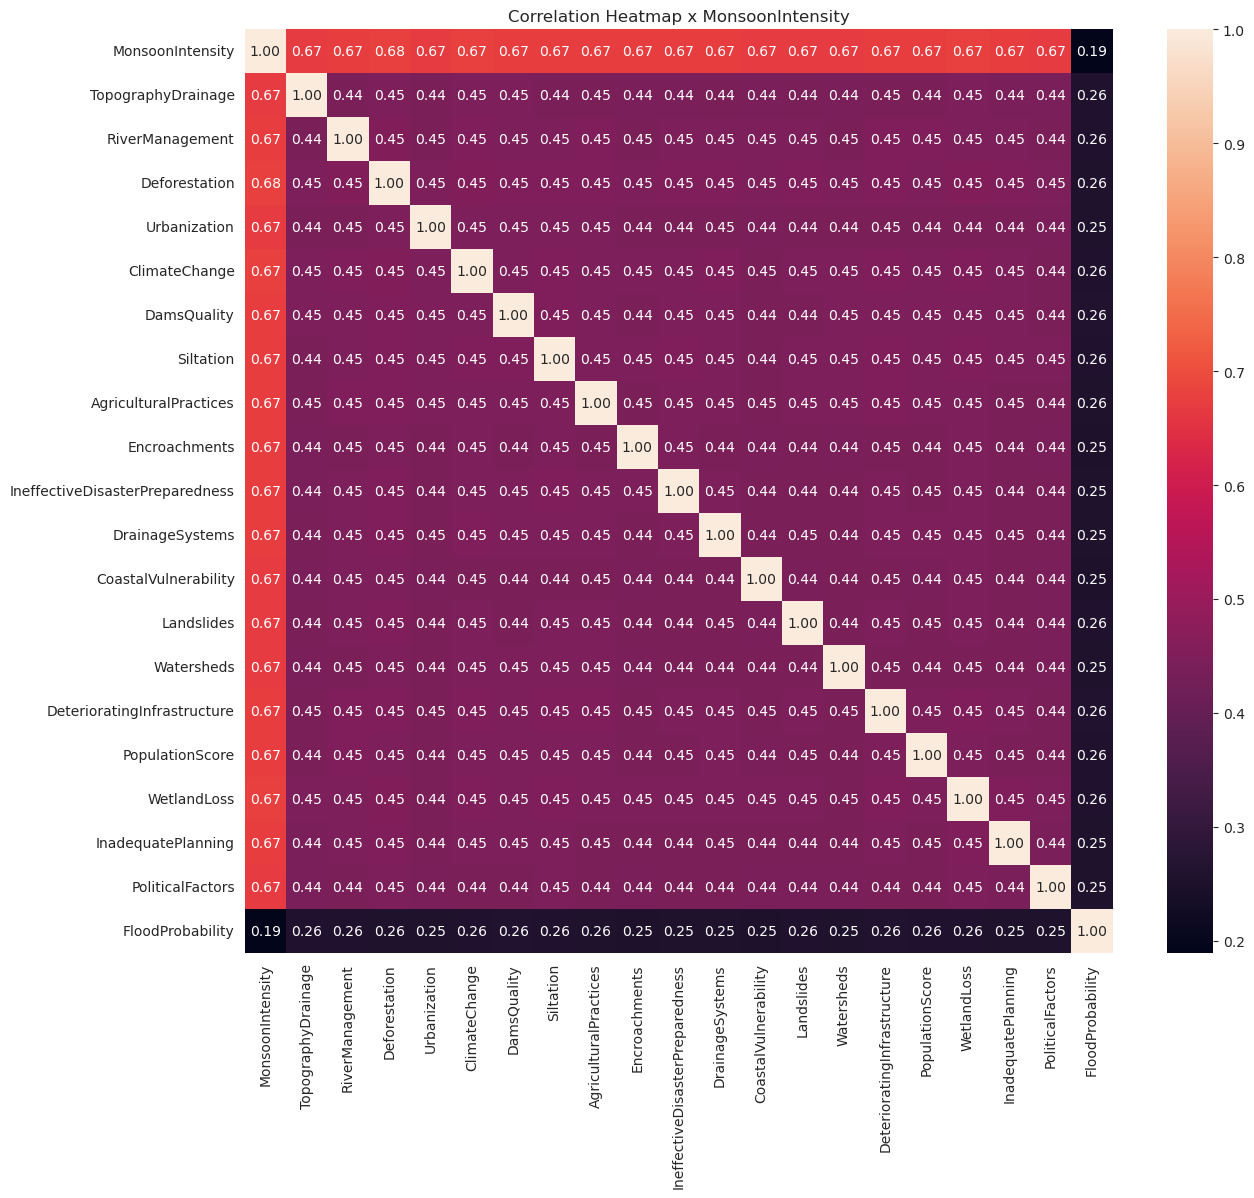
\includegraphics[width=7cm]{./images/heatmap2.png}
			\captionof{figure}{نقشه گرمایی همبستگی متغیرها در صورت ضرب ستون MonsoonIntensity در همه‌ی ستون‌های دیگر به‌جز خودش و FloodProbability}
\end{center}
		\subsection{اسکیل کردن}
		در این قسمت ما از اسکیلر استاندارد و اسکیلر کمینه بیشینه استفاده کردیم.
		\subsection{آماده‌سازی داده‌ها برای آموزش مدل}	
داده‌ها را به صورت ۴ مجموعه داده در حالت‌های مختلف با اسکیلرهای مختلف آماده کردیم و متغیرهای وابسته‌ی آن را از متغیر مستقل آن جدا کردیم. سپس یک بردار تصادفی از وزن‌ها (slope) و یک بردار تصادفی از مقادیر ثابت (intercept) آماده کردیم تا نتایج حاصل از مدل را در آن بریزیم.
\section{مدل‌سازی داده‌ها و آموزش}
در این قسمت ما به مدل‌سازی داده‌ها و پیش‌بینی می‌پردازیم.
\subsection{تابع رگرسیون خطی}
\paragraph{تابع هزینه}
این تابع در اول کدنویسی بسیار ساده بود اما با اضافه شدن سایر ویژگی‌ها کمی به پیچیدگی آن افزوده شد.
در این تابع تعدادی ایپاک از کاربر دریافت می‌شود. سپس مشتق خطای هر سطر نسبت به مقدار واقعی محاسبه می‌شود. تابع خطای ما در اینجا مشتق تابع میانگین مربع خطاست که ما را به نقطه‌ی بهینه هدایت می‌کند.
\paragraph{تکانه}
 ما در اینجا یک velocity تعریف کردیم که برای اینکه تکانه واقعا تغییر کند، در اینجا به‌جای اینکه خطا مستقیما روی slope اثر بگذارد (با \lr{learning rate} مشخص)، از سرعت قبلی هم کاملا اثر می‌پذیرد و این کمک می‌کند از داده‌های outlier کمتر اثربپذیریم و سریع‌تر به چیزی که می‌خواهیم میل کنیم.برای مثال با تکانه کم، ما حدود ۶۰۰ تکرار نیاز داشتیم تا زودهنگام به نتیجه برسیم اما با پیاده‌سازی تکانه این عدد به ۳۴۰ هزار رسید و زمان را به نصف کاهش داد!
 \paragraph{توقف زودهنگام}
مسئله‌ی بعدی که قبل‌تر هم به آن اشاره شد خروج زود هنگام است. قبل از پیاده‌سازی این عملکرد، زمان اجرای یک دور تابع جبرخطی برای ۴ مجموعه داده حتی با وجود اینکه نمودارها جدا رسم می‌شدند برای ۱۰ ایپاک چیزی حدود ۶ دقیقه و نیم بود! اما با پیاده‌سازی این تابع، با حفظ عملکرد، تابع آموزش در کمتر از ۱۰ ثانیه هر ۴ مدل را آموزش می‌داد!
\paragraph{عادی‌سازی}
هرچند تکنیک عادی‌سازی 
 \href{https://medium.com/@alejandro.itoaramendia/l1-and-l2-regularization-part-2-a-complete-guide-0b16b4ab79ce}{\lr{L2} }
در کد پیاده‌سازی شد که باعث می‌شود خود گردیان با مقادیر قبلی slope جمع شود ولی نتیجه‌های این اتفاق باعث می‌شد توابع underfit شود و اصلا به چیزی که می‌خواهیم شبیه نشود. یعنی با پیاده‌سازی این مکانیسم، امتیاز
\lr{$R^{2}$}
روی داده‌های تست به کمتر از ۸٫۰ می‌رسید که این از نظر ما مطلوب نبود. هرچند در کارکرد فلسفه‌ی آن هم همین است.
\paragraph{تغییر سرعت یادگیری}
ما  از یک تکنیک ساده استفاده کردیم که در آن نرخ یادگیری بعد از هر ایپاک در یک مقدار کمتر از ۱ ضرب می‌شود. این با این فرض درنظر گرفته شده که مدل از جایی به بعد همگرا می‌شود. بیش از اندازه کوچک بودن این مقدار باعث می‌شود مدل underfit شود.
\paragraph{نمونه‌برداری}
سیاست ما این بود به‌جای مقایسه‌ی ایپاک‌ها برای توقف زودهنگام و همچنین به‌جای رسم همه‌ی تکرارها از نمونه‌برداری بین  تعدادی سطر استفاده کنیم. بدین منظور میانگین خطای هر مثلا ۱۰۰۰ خط را اندازه‌گیری می‌کردیم و سپس بعد هر هزار بار آن را صفر می‌کردیم.
\paragraph{رسم تغییرات‌}
در اینجا ما کلیه تغییرات را بر حسب ایپاک و تکرار همچنین تغییرات سرعت یادگیری و خطا را نشان داده‌ایم.
\section{پیش‌بینی}
در این بخش، داده‌های آموزش و آزمون را به مدل می‌دهیم. تبعا به دنبال مدلی هستیم که روی هر دو داده‌ی آموزش و آزمون مقدار
\lr{$R^{2}$}
 کافی برای ما فراهم کند. 
\begin{center}
	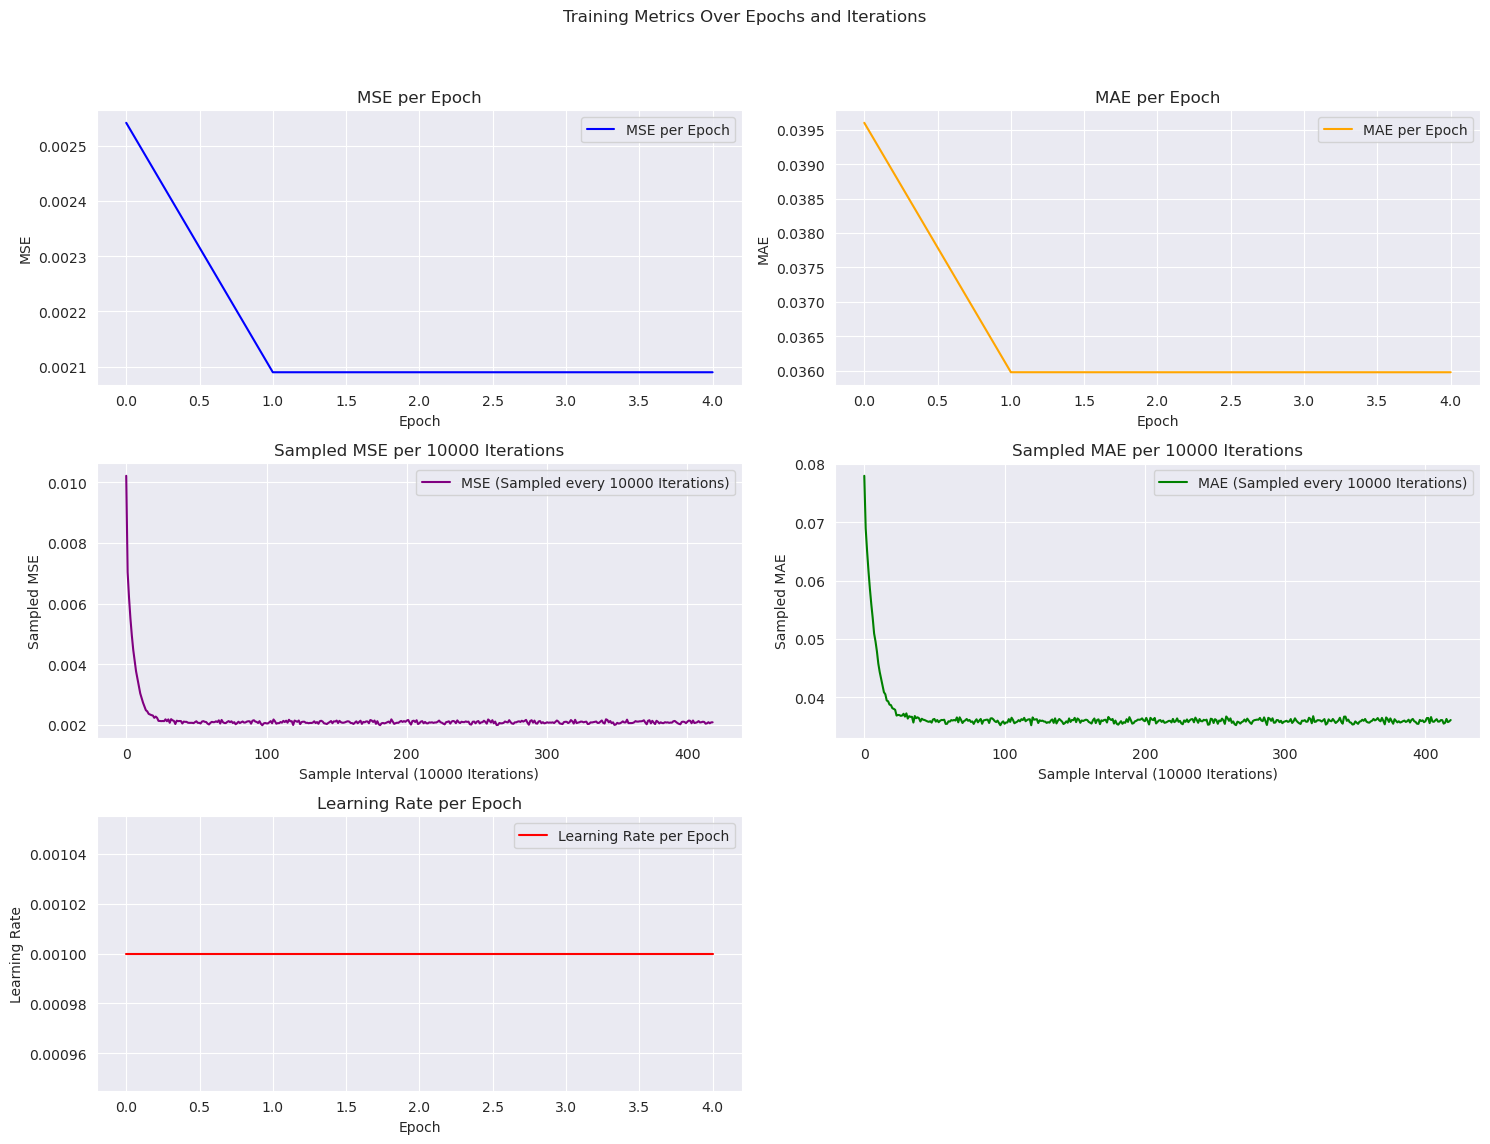
\includegraphics[width=12cm]{./images/train_minmax.png}
	\captionof{figure}{	آموزش داده‌های اسکیل شده با کمینه بیشینه در حالت پایه با ۵ ایپاک و سرعت آموزش ۰۱٫۰}
\end{center}
\begin{center}
	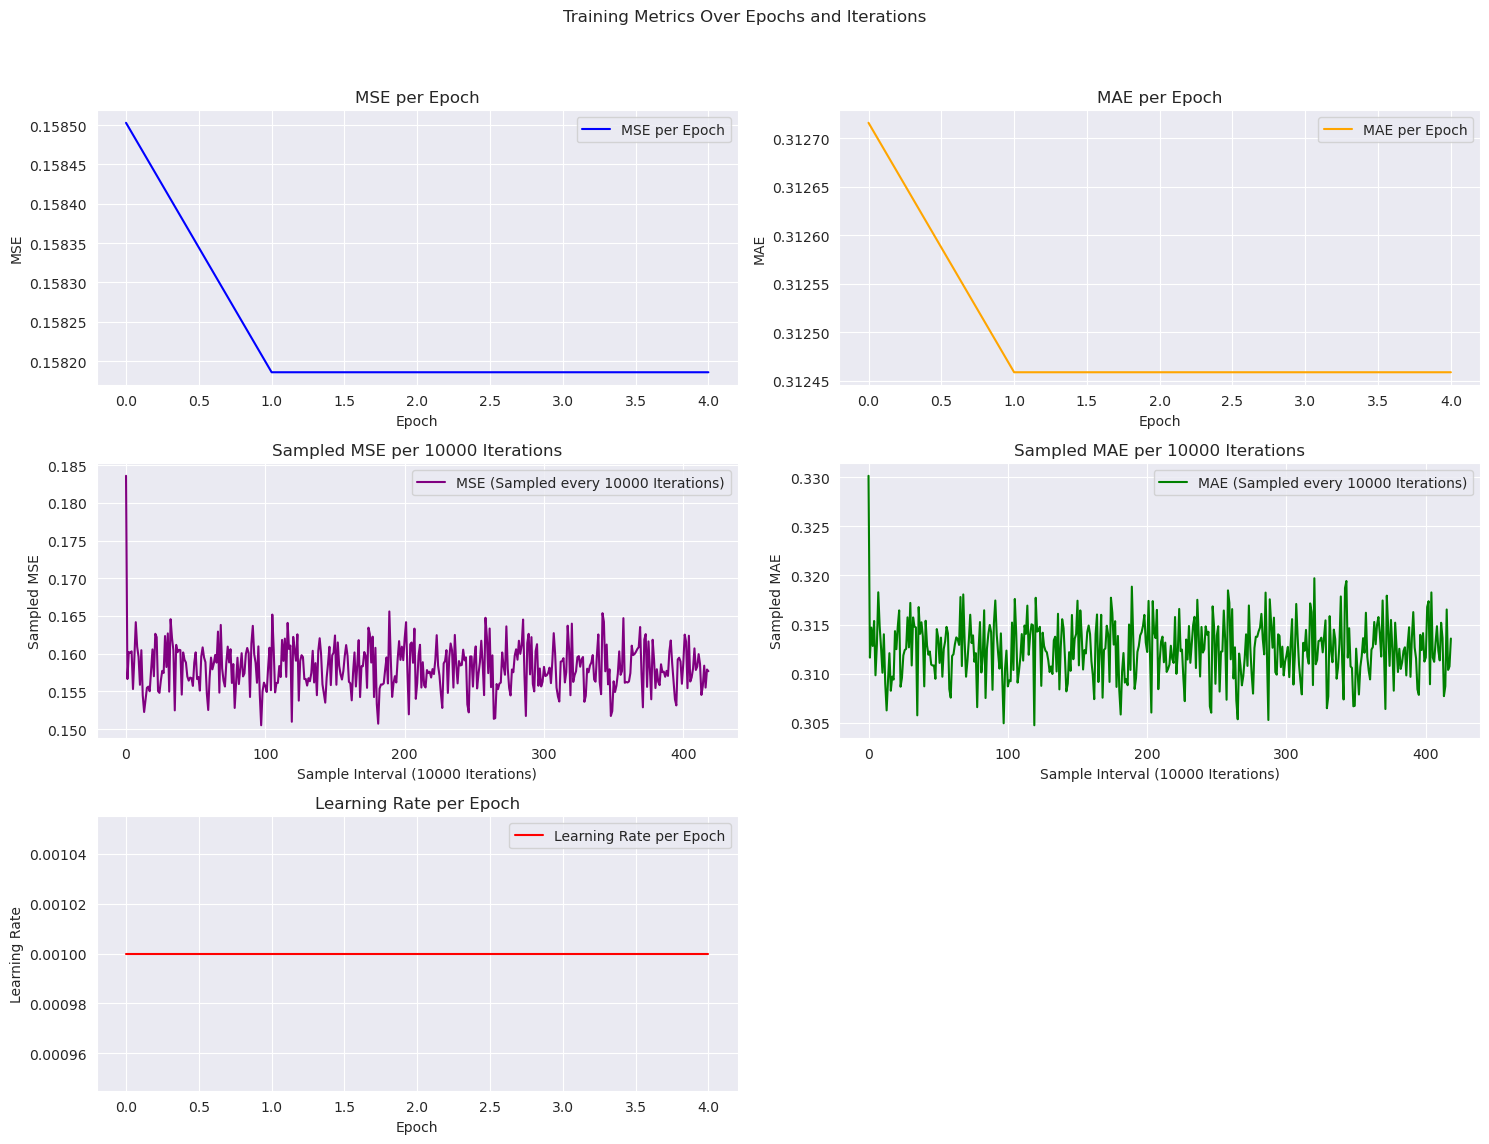
\includegraphics[width=12cm]{./images/train_z.png}
	\captionof{figure}{	آموزش داده‌های اسکیل شده با z  در حالت پایه با ۵ ایپاک}
\end{center}

\subsection{پیش‌بینی روی داده‌های تست}
برای داده‌های تست فرآیند مشابهی در زمینه‌ی اسکیل کردن طی می‌کنیم. در اینجا باید اشاره کنیم از همان اسکیلرهای آموزش استفاده می‌کنیم. سپس این داده‌ها را به مدل‌ها می‌دهیم و پیش‌بینی آن‌ها را می‌سنجیم. خروجی:
\par

\begin{LTR}
	\begin{minted}[frame=lines, fontsize=\small, tabsize=4, texcomments=false, breaklines=true, breakanywhere=true]{text}
Mean Absolute Error: 0.31429430780462186
Mean Squared Error: 0.15990997244596597
R2 Score: 0.839718589887849

Mean Absolute Error: 0.036034161275208226
Mean Squared Error: 0.0020939675495502044
R2 Score: 0.8440392259660622

Mean Absolute Error: 0.3122935770427608
Mean Squared Error: 0.15784894281081954
R2 Score: 0.8417844068669359

Mean Absolute Error: 0.03595022487165275
Mean Squared Error: 0.002089504719597371
R2 Score: 0.8443716219547084
	\end{minted}
\end{LTR}



\subsection{بازی کردن با پارامترها}
در نهایت ما می‌توانیم با بازی کردن با پارمترهای تابع رگرسیون در زمان کوتاه به توابع بسیار خوبی برسیم. نمونه‌ی این تابع:
\begin{center}
	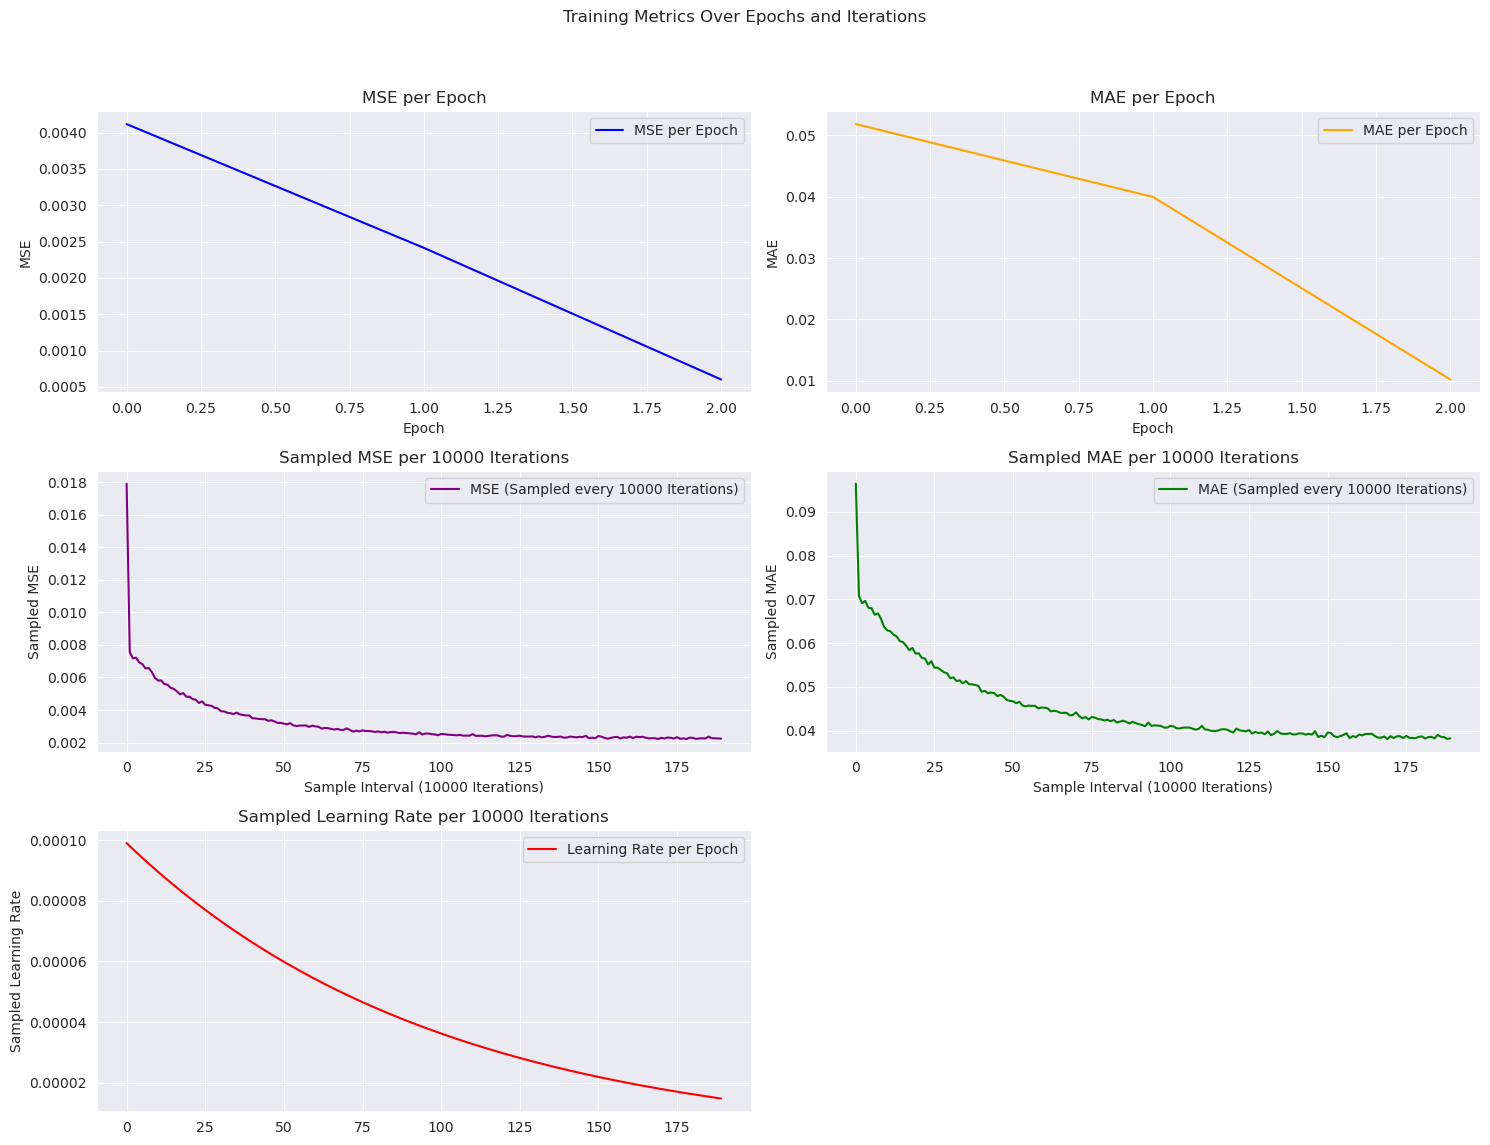
\includegraphics[width=12cm]{./images/train2.png}
	\captionof{figure}{\lr{Early stopping at iteration 2370000 with MSE: 0.002220466560191889}}
\end{center}
که در آن پارامترها به نحو زیر تعیین شده بودند:
\begin{LTR}
	\begin{minted}[frame=lines, fontsize=\small, tabsize=4, texcomments=false, breaklines=true, breakanywhere=true]{python}
epochs_number=10
initial_learning_rate=0001.0
momentum=5.0
patience=20
regularization_param=0.0
lr_decrease=99.0
iteration_sample=10000
	\end{minted}
\end{LTR}

که درظرف ۱۵ ثانیه آموزش مدل به نتایج زیر رسیدیم:
\begin{LTR}
	\begin{minted}[frame=lines, fontsize=\small, tabsize=4, texcomments=false, breaklines=true, breakanywhere=true]{text}
Mean Absolute Error: 0381413675044361.0
Mean Squared Error: 0022375861525931085.0
R2 Score: 8333423703719746.0
	\end{minted}
\end{LTR}

\end{document}